
\newcommand{\pull}[3]{
\begin{frame}{Pull distribution for #3}
\includegraphics[width=\textwidth]{2020_05_14/figs/antiSym_#1/antiSym_#1/4/pulls/#2.png}
\end{frame}
\begin{frame}{Status for #3}

\includegraphics[width=\textwidth]{2020_05_14/figs/antiSym_#1/antiSym_#1/4/pulls/#2_Status.png}
\end{frame}

}

\newcommand{\pullz}[3]{
\begin{frame}{Pull distribution for #3}
\includegraphics[width=\textwidth]{2020_05_14/figs/antiSym_#1/antiSym_#1/4/pulls/#2.png}
\end{frame}

}


\newcommand{\pulls}[2]{
    \pull{#1}{Comb}{Combined Tag #2}
    \pull{#1}{KK}{$\KK$ tag #2}
    \pull{#1}{Kspi0}{$\Kspiz$ tag #2}
    \pull{#1}{Kppim}{$\Kppim$ tag #2}
    \pull{#1}{Kmpip}{$\Kmpip$ tag #2} 
    \pull{#1}{Kspipi}{$\Kspipi$ tag #2}
}

\newcommand{\pullzs}[2]{
    \pullz{#1}{Comb}{Combined Tag #2}
    \pullz{#1}{KK}{$\KK$ tag #2}
    \pullz{#1}{Kspi0}{$\Kspiz$ tag #2}
    \pullz{#1}{Kppim}{$\Kppim$ tag #2}
    \pullz{#1}{Kmpip}{$\Kmpip$ tag #2} 
    \pullz{#1}{Kspipi}{$\Kspipi$ tag #2}
}

\newcommand{\projod}[5]{
    \begin{frame}{Projection for #5}


        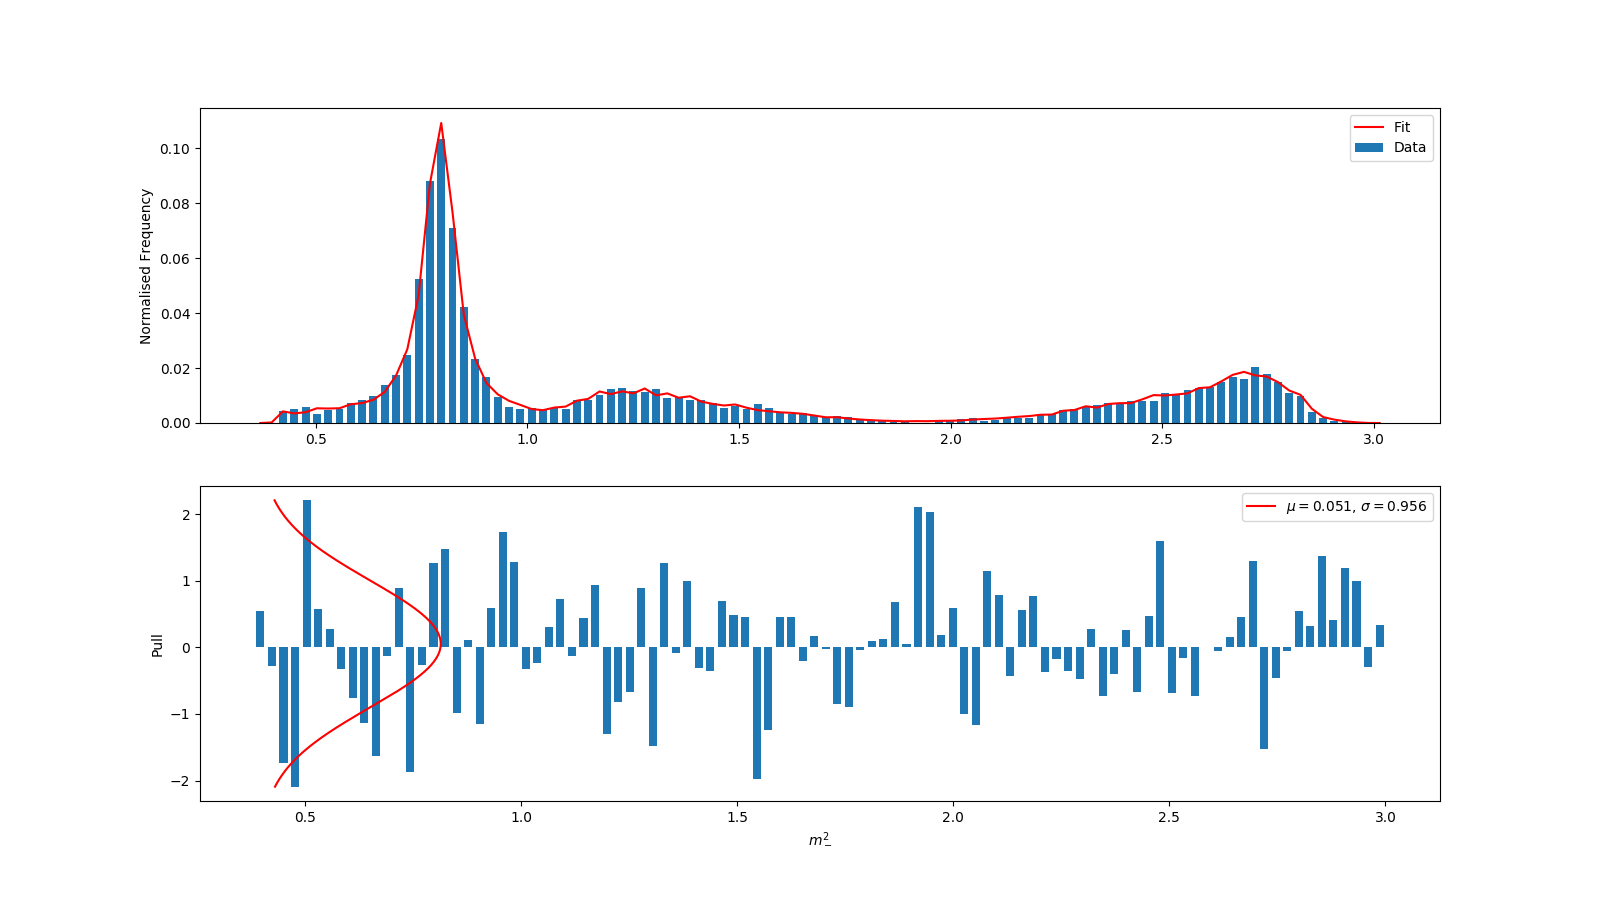
\includegraphics[width=\textwidth]{2020_05_14/figs/antiSym_#1/antiSym_#1/proj/#2/#3/#4/s01.png}

    \end{frame}

    \begin{frame}{Projection for #5}
            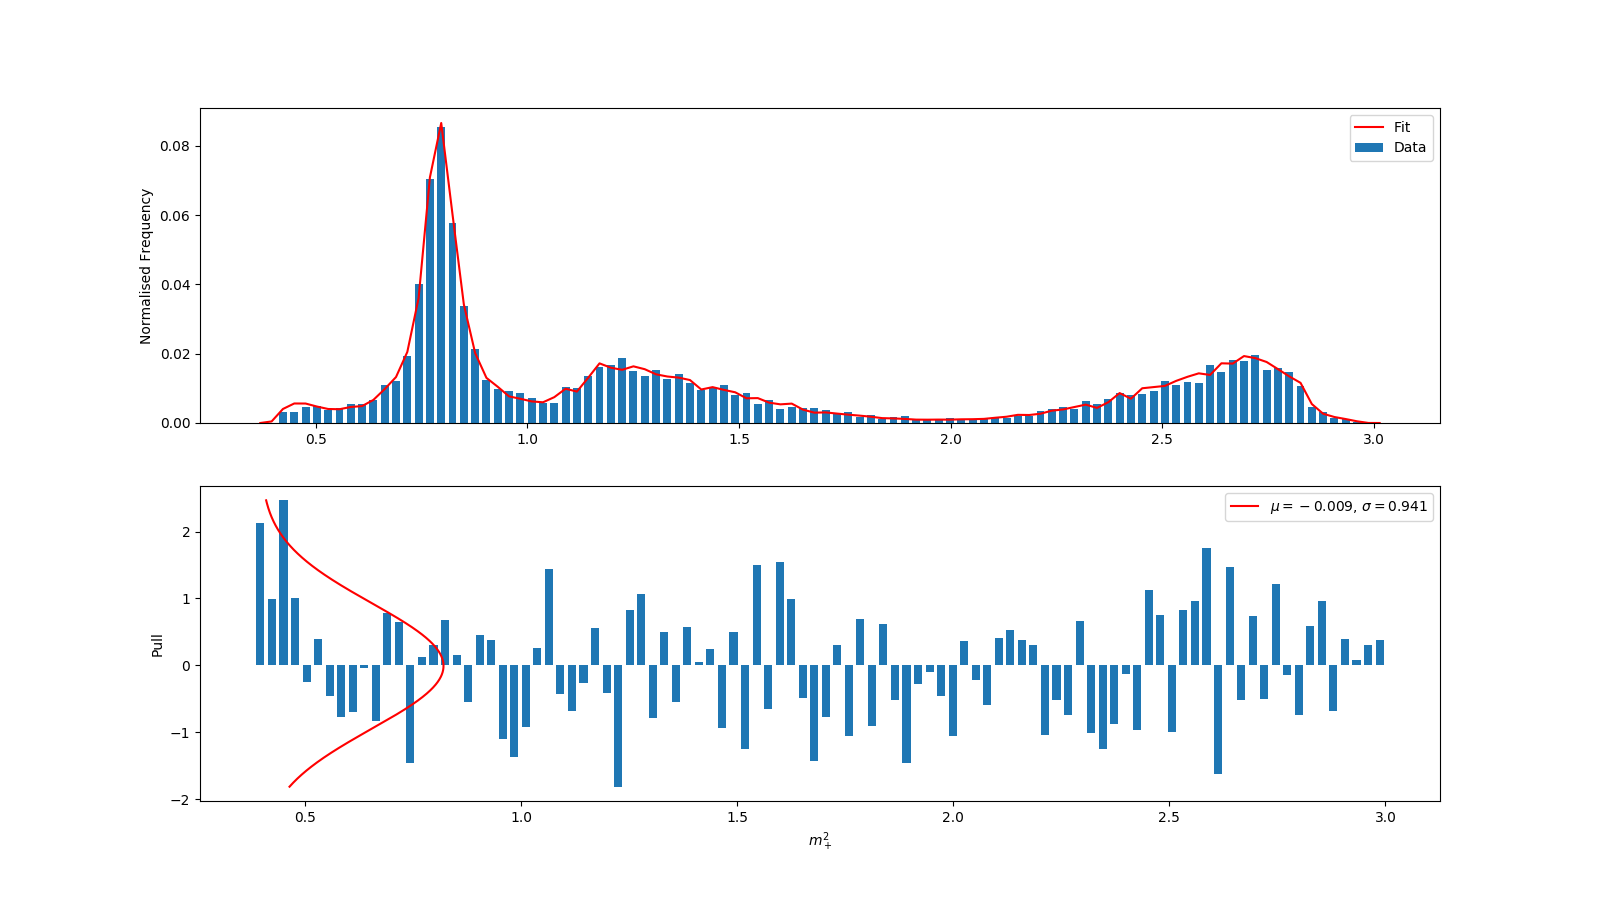
\includegraphics[width=\textwidth]{2020_05_14/figs/antiSym_#1/antiSym_#1/proj/#2/#3/#4/s02.png}

   

    \end{frame}
}

\newcommand{\projtd}[5]{
    \begin{frame}{Projection for #5}


                \includegraphics[width=\textwidth]{2020_05_14/figs/antiSym_#1/antiSym_#1/proj/#2/#3/#4_s01_vs_s02.png}

    \end{frame}
    \begin{frame}{Projection for #5}

                \includegraphics[width=\textwidth]{2020_05_14/figs/antiSym_#1/antiSym_#1/proj/#2/#3/#4_s01_vs_s02_pull.png}


    \end{frame}

}




\newcommand{\allprojod}[3]{
    \projod{#1}{#2}{#3}{KK}{s01}
    \projod{#1}{#2}{#3}{Kspi0}{s01}
    \projod{#1}{#2}{#3}{Kppim}{s01}
    \projod{#1}{#2}{#3}{Kmpip}{s01}
    \projod{#1}{#2}{#3}{Kspipi}{s01}

}
\begin{frame}{Overview}
    \begin{itemize}
        \item Previously had issues when constraining $C_{ij}$ at higher order - effectively killing off higher order corrections to $\dd$.
        \item Reran pull studies with zero constraints on $C_{ij}$.
        \item Examined the distribution of fit status from jobs on the grid (are we converging cleanly?)
        \end{itemize}
\end{frame}

\begin{frame}{Fit Status}
    From \texttt{Minuit2} (see \url{https://root.cern.ch/root/html/ROOT__Minuit2__Minuit2Minimizer.html})
    \begin{enumerate}
        \item Status 0 - fit is converged
        \item Status 1 - The Covariance matrix was made positive definite 
        \item Status 2 - The Hessian matrix is invalid 
        \item Status 3 - The \texttt{edm} was above maximum
    \end{enumerate}
    Ideally we get status 0 for every fit, but we see many status 1 and 3 when using the Grid.
    Solution : Redo the fits until we get to a minimum (status 0) (up to some number of retries - say 5).
    Test this with a smaller order, it takes significantly longer to converge with more parameters. At $N_\text{order}=4$ we have 10 parameters.
\end{frame}
\pulls{simple}{Pulls for Anti-symmetric polynomial with all statuses}
\pullzs{simple0}{Pulls for Anti-symmetric polynomial with only status 0}
%\pulls{simple0}{Pulls for Anti-symmetric polynomial with only status 0 and 1}
\projod{simple}{139}{7}{Kspipi}{Projection for status 0}
\projtd{simple}{139}{7}{Kspipi}{2D projection for status 0}

%\projod{simple}{143}{0}{Kspipi}{Projection for status 1}
%\projtd{simple}{143}{0}{Kspipi}{2D projection for status 1}

\projod{simple}{142}{4}{Kspipi}{Projection for status 3}
\projtd{simple}{142}{4}{Kspipi}{2D projection for status 3}
